\documentclass[border=4pt]{standalone}
\usepackage{amsmath,amssymb}
\usepackage{tikz}
\begin{document}
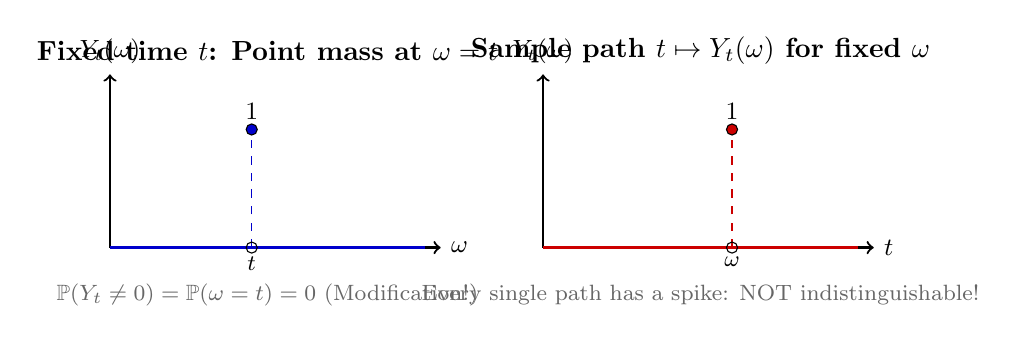
\begin{tikzpicture}[font=\small]
  % Fixed t view
  \begin{scope}[xshift=0cm]
    \node[font=\bfseries] at (2.0, 2.5) {Fixed time $t$: Point mass at $\omega = t$};
    \draw[->, thick] (0,0) -- (4.2,0) node[right] {$\omega$};
    \draw[->, thick] (0,0) -- (0,2.2) node[above] {$Y_t(\omega)$};
    \draw[very thick, blue!80!black] (0,0) -- (1.8,0);
    \draw[very thick, blue!80!black] (1.8,0) -- (4.0,0);
    \draw[fill=blue!80!black] (1.8, 1.5) circle (2pt) node[above] {$1$};
    \draw[dashed, blue!80!black] (1.8, 0) -- (1.8, 1.5);
    \draw (1.8, 0) circle (2pt);
    \node[below, font=\footnotesize] at (1.8,0) {$t$};
    \node[font=\footnotesize, text=gray!80!black] at (2.0, -0.6) {$\mathbb{P}(Y_t \ne 0) = \mathbb{P}(\omega = t) = 0$ (Modification!)};
  \end{scope}

  % Fixed omega view
  \begin{scope}[xshift=5.5cm]
    \node[font=\bfseries] at (2.0, 2.5) {Sample path $t \mapsto Y_t(\omega)$ for fixed $\omega$};
    \draw[->, thick] (0,0) -- (4.2,0) node[right] {$t$};
    \draw[->, thick] (0,0) -- (0,2.2) node[above] {$Y_t(\omega)$};
    \draw[very thick, red!80!black] (0,0) -- (2.4,0);
    \draw[very thick, red!80!black] (2.4,0) -- (4.0,0);
    \draw[fill=red!80!black] (2.4, 1.5) circle (2pt) node[above] {$1$};
    \draw[dashed, red!80!black] (2.4, 0) -- (2.4, 1.5);
    \draw (2.4, 0) circle (2pt);
    \node[below, font=\footnotesize] at (2.4,0) {$\omega$};
    \node[font=\footnotesize, text=gray!80!black] at (2.0, -0.6) {Every single path has a spike: NOT indistinguishable!};
  \end{scope}
\end{tikzpicture}
\end{document}